% !TEX root = ../my-thesis.tex
%
\chapter{Etat de l'art}

% TODO : S'assurer que les différentes catégories scientifiques sont là
% TODO : Vérifier qu'il y a bien une justification vers un choix de progression et des parties dé-corélées sans fil conducteur.

\cleanchapterquote{Un petit chapitre pour le doctorant, un grand chapitre pour l'humanité}{Doctorant anonyme}{(Citation temporaire)}

\section{Segmentation}
\label{sec:EA:segmentation}

% Porte d'entrée par la visualisation de données

Après l'acquisition des images provenants des systèmes d'IRM et de Tomodensitométrie, se pose la question de la visualisation des données. En effet, les images obtenues sont des matrices 3D et une visualisation 3D naïve ne permet de discerner que l'enveloppe extérieure d'un volume. Parmis les techniques de visualisation, la plus simple et la moins coûteuse, revient à considérer le volume 3D comme une suite de coupes 2D. On peut ainsi visualiser la totalité des tissues d'un volume de manière itérative. Cette méthode oblige cependant les médecins à une gymnastique mentale pour reconstituer, dans leur esprit, l'organe 3D étudié. Une autre méthode consiste à visualiser les objets les plus saillants de l'image. La technique la plus utilisée, la MIP (maximum intensity projection), consiste à lancer pour chaque pixels d'un plan $p_i$, un rayon traversant le volume de donnée. L'intensité maximale des voxel le long de ce rayon est ensuite assignée à $p_i$. Cette méthode à l'avantage de faire ressortir les éléments les plus intenses de l'image et convient particulièrement à des structures mis en valeur par un agent de contraste. Elle est aussi très simple à implémenter et est peu coûteuse en ressources de calcul. Cependant, cette méthode fait perdre toute perception de profondeur, à cause de la projection, ce qui peut perturber l'analyse des structures. Ce dernier désavantage peut toutefois être contourné par l'utilisation d'une MIP dans une scène 3D contenant le volume 3D de l'image et une camera. La projection s'effectuant alors sur le plan de la caméra et il est possible de déplacer l'observateur autour du volume qui permet grâce au mouvement de rétablir implicitement cette information de profondeur. L'utilisation de la MIP pour l'étude d'un organe, peut tout de fois être parasité par des organes adjacents plus intenses, comme par exemple les os de la cage toracique.

A noter que ces deux méthodes ne sont pas invasives, dans le sens où aucune transformation n'est appliquée à l'image originale.

\begin{figure}
  \centering
  
\includegraphics[height=3cm]{Images/img_required.jpg}
  \label{fig:visualisation en coupe}
  \caption{visualisation en coupe}
\end{figure}

\begin{figure}
  \centering
  
\includegraphics[height=3cm]{Images/img_required.jpg}
  
\includegraphics[height=3cm]{Images/img_required.jpg}
  \label{fig:visualisation MIP}
  \caption{Maximaly intensity projection (mip). L'intensité maximale est rétroprojeté le long du rayon sur le plan d'origine. La MIP peut s'effectuer en utilisant les bords de l'image, où le plan de la caméra dans une scène 3D}
\end{figure}

Bien que la vue en coupes 2D et la MIP offrent une visualisation convenable dans de nombreux cas, celles-ci peuvent se révéler insuffisante pour la représentation de structures complexes ou pour des tâches de mesures volumétriques. Dans ce cas, il est nécessaire d'extraire les structures d'intérêts de l'information superflux qui les entourent. C'est ce processus d'extraction que l'on nomme segmentation.  


\subsection{Segmentation classique}
\label{sec:EA:segmentation_historique}
% Etat de l'art de la segmentation hiérarchisée par problématique
% contraste
% formea
% 
L'automatisation de la segmentation pour les images médicales est une tâche complexe. Elle doit répondre à des problématiques variées, provenant à la fois des conditions d'acquisition de l'image \ref{sec:contexte:images}, de forme de l'organe et de l'extraction d'éléments sémantiques haut niveau. Ces contraintes peuvent mener à l'élaboration de chaines de traitements proposant un nombre d'étapes importants. Ainsi, Marcan \cite{Marcan2014_vessel_seg} propose un pipeline de segmentation en 16 étapes mélangeant, filtrage du bruit, sélection des éléments pertinents par masques et analyses des composantes connexes pour la segmentation des vaisseaux du foie. Goceri \cite{Goceri2017_vessel} propose une méthode en 14 étapes aliant partions en régions d'intérêts et étirement du contraste (contrast stretching) afin de différencier vaisseaux hépatiques des tissues du foie.

Une taxonomie précise des méthodes de segmentation est difficile à établir tant les publications présentent différentes combinaisons de briques algorithmiques. Lesage \cite{Lesage2009_review} propose une décomposition des étapes de segmentation sous la forme de 3 grands thèmes : Les modèles d'intensités et modèles géométriques, les descripteurs d'images et les schéma d'extractions. Les modèles constituent l'ensemble des hypothèses permettant d'identifier l'objet à segmenter. Les descripteurs reposent sur des caractéristiques spécifiques de l'image qui permettent de mesurer l'écart de similarité entre les données et le modèle. Enfin, le schéma d'extraction permet de choisir le seuil idéal de segmentation en fonction des caractéristiques de l'image et du/des modèle(s) choisi(s).

Dans cette partie, nous explicitons les briques algorithmiques classiquement utilisées pour la segmentation des vaisseaux. Nous prenons comme parti pris d'explorer le pipeline à l'envers, c'est à dire, de présenter les schémas d'extractions courants, puis les descripteurs communéments utilisées pour finir par les modèles de représentations. Nous pourrons ainsi ammener progressivement le rehaussement de vaisseaux qui se trouve à cheval entre les deux dernières catégories.

\subsubsection{Schéma d'extraction}

Une segmentation est avant tout une méthode permettant de classifier si un pixel appartient à un objet d'intérêt. Les schémas d'extractions proposent un ensemble de cadres pour automatiser ce choix.

\paragraph{Courbes de niveaux}
La méthode des courbes de niveau (level set) permet à l'origine de simuler la propagation d'une onde ou d'un fluide dans un milieu. Appliquée à la segmentation, elle permet de faire s'étendre en fonction du temps un contour jusqu'à ce qu'un critère d'arrêt soit atteint. Ce critère d'arrêt est souvent exprimé comme une énergie à minimiser. Le suivi d'un contour évoluant avec le temps est une tâche non triviale, notamment lorsque la topologie du contour change. C'est par exemple le cas lorsqu'un contour se divise en deux contours distincts. Les levels sets permettent de contourner ce problème en définissant un contour implicite comme l'intersection de deux surfaces. La première surface correspond à l'image vue comme une carte de hauteur et la seconde courbe $\phi$ correspond aux critère de partition. La dynamique d'évolution du contour implicite est géré par l'élévation de la courbe $\phi$ en fonction du temps.

\begin{figure}
  \centering
  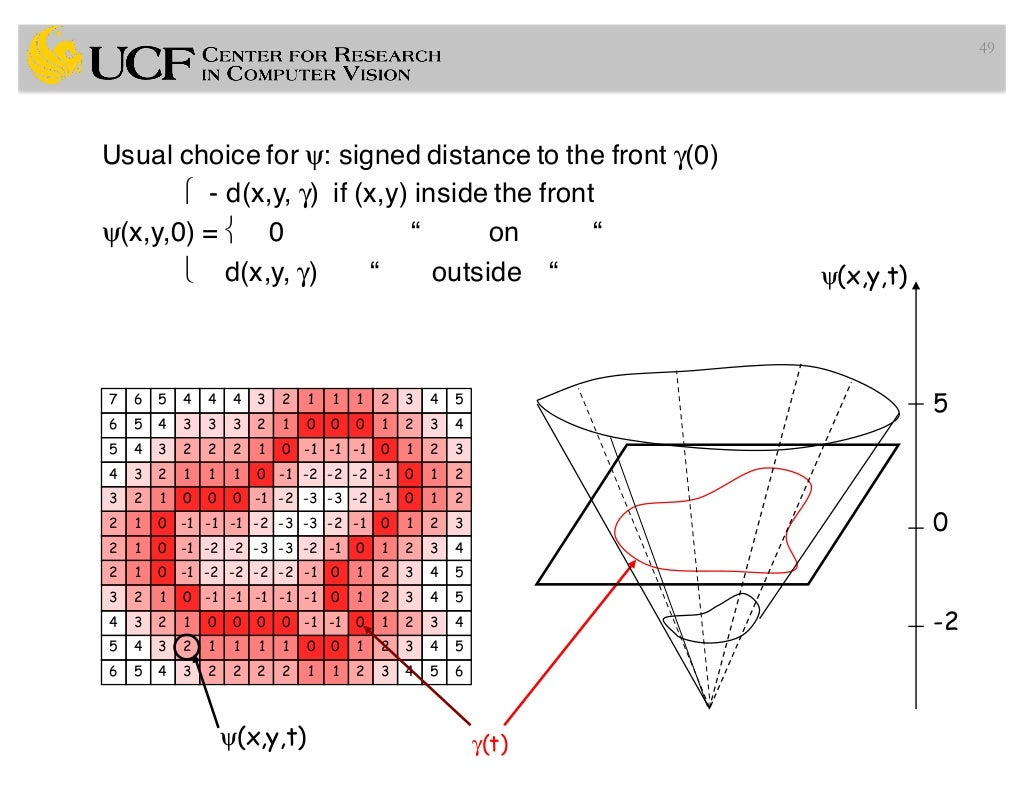
\includegraphics[height=3cm]{Images/level_set_active_contour.jpeg}
  \label{fig:Courbes de niveaux}
  \caption{Courbes de niveaux}
\end{figure}

Li \cite{Li2011_mri_level_set} utilise les levels set pour segmenter un objet malgrès des intensités non homogènes, pour cela il définit un critère de classification local au voisinage des pixels afin d'estimer un champ de biais d'intensité qui est ensuite incorporé dans l'énergie de propagation. Zeng \cite{Zeng2018_liver_hybrid_active_contour_region_growing} utilise une méthode de contour actifs (spécification du level set) dont le critère est estime à la fois la cohérence entre les régions délimités par le contour et une carte de contours basée sur le gradient.

\paragraph{Graph cut}

Une image peut-être représentée sous la forme d'un graphe. Dans ce graph, les noeuds sont les pixels et les arêtes encodent une relation de similarité entre les pixels. Cette relation peut être spatiale où plus complexe. Dans ce contexte, segmenter un objet ou une région revient à trouver la coupure qui maximise la vraissemblance à l'intérieur de chaque partition et minimise la vraissemblance entre deux partitions relativement à un critère.

Zeng \cite{Zeng2017_liver_oof_graph_cut} propose un rafinement par graph cut d'une segmentation initiale, en utilisant un critère de région basé sur la vraisemblance logarithmique (negative log likelyhood) et un critère de bordure basé sur le flux (voir SEC. \ref{modèles ou rehaussement}).

\begin{figure}
  \centering
  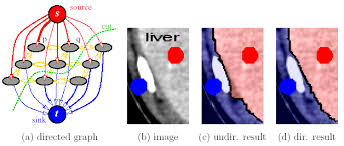
\includegraphics[height=3cm]{Images/graph_cut.jpeg}
  \label{fig:Graph cut}
  \caption{Graph cut, le graph cut nécessite des graines afin de définir les deux régions à rafiner}
\end{figure}

Le choix d'une délimitation entre fond et segmentation n'est pas toujours aisé, en particulier dans les images médicales où les bords des objets à segmenter sont assez mal définis. La théorie des ensembles floues permet de modéliser cette incertitude. Au lieu d'associer une classe binaire aux pixels, on associe à chaque pixel un ( A développer, car pas clair...)

\cite{Zhang2018_liver_fuzzy_connectedness}
\cite{Caponetti2014_fuzzy_morphology}
\cite{Radojevic2015_fuzzy_logic}
\cite{Sigurosson2014_retinal_morpho_fuzzy}

\subsubsection{Caractéristiques}

Les caractéristiques extraites de l'image permettent de fournir des descripteurs quantifiables qui peuvent être incorporés dans les schémas d'extractions vus à la section précédente.

Les caractéristiques les plus employés sont les caractéristiques différencielles. Celles-ci permettent d'étudier les variations de dynamiques dans l'image et permettent notament d'extraire des informations géométriques locales.

Le premier descripteur différentiel est la dérivée première, aussi appelé gradient. Celui-ci peut-être calculé de différentes manières (différences finies, convolution de noyau gaussiens dérivés, etc.) et fourni une information sur la variation des intensités des pixels au niveau local. Le gradient est une quantité scalaire et s'exprime comme la somme des dérivées partielles de l'image. Là où le gradient permet de quantifier les changements d'intensités, l'utilisation des dérivées partielles sous forme de champ de vecteurs gradients, permet d'obtenir une information de direction du gradient. En particulier, une représentation compacte de l'orientation de la géométrie locale autour d'un pixel est le tenseur de structure.

\begin{equation}
  T = definition d'un tenseur de structure ici
\end{equation}

La dérivée seconde permet d'obtenir des informations sur la courbure local de l'image autour d'un pixel. Le laplacien, qui s'exprime comme la divergeance du gradient, permet d'évaluer la ressemblance du voisinage local à une sphère. \cite{Wang2020_tensor_cut}

Tout comme pour le gradient, le laplacien est une quantité sans information de direction, on utilise la matrice des dérivées partielles secondes, la hessienne, pour encoder les informations de direction.

Emprunté aux la théorie des probabilités, les moments permettent aussi de décrire la dispersion d'une variable aléatoire (en l'occurence, l'intensité du voisinage d'un pixel), permet d'obtenir des informations sur l'espérance, la variance, l'assymétrie, etc. Ceux-ci se définissent par :

\begin{equation}
  T = definition d'un moment ici
\end{equation}

Adossés aux champs de vecteurs gradients et aux modèles, les caractéristiques de flux permettent d'étudier la dynamique d'intensité autour des contours d'un objet. Ces descripteurs nécessitent un choix préalable d'un modèle géométrique d'objet à segmenter et sont relativement rigides.

\subsubsection{Modèles}

La définition de modèles pour l'objet à segmenter nous permet de mesurer la fidélité d'une région décrite par des caractéristiques.

Les modèles sont en général au nombre de trois, les modèles d'intensités, les modèles géométriques et les modèles à base d'atlas.

Les modèles d'intensités sont construits sur l'intensité prédites des structures à segmenter. Pour l'angiographie, une des hypothèse de base est que les vaisseaux ont une intensité différente des tissues qui les entourent. En particulier pour l'angiographie avec agent de contraste, les vaisseaux sont supposés clairs sur fond foncé. Dans le cas contraire, e.g vaisseaux foncés sur fond clair, il suffit d'inverser les niveaux de gris de l'image pour retomber sur l'hypothèse initiale.

Les modèles d'intensités peuvent être construit en amont ou iterativement au cours de la segmentation. He \cite{He2013_multi_otsu} propose une segmentation itérative par seuillage automatiques Otsu et étirement de contraste afin d'élargir peu à peu le modèle d'intensité sous jacent. Bukenya \cite{bukenya2016_heart_otsu_top_hat_hessian}, étend cette méthode à la 3D et la renforce avec des modèles géométriques afin de faciliter la détection des petits vaisseaux de faible intensité, De la même manière BahadarKhan, utilise une méthode hybride \cite{Bahadarkhan2016_fundus_region_based_otsu}.

Parmis les méthodes qui tirent parti des modèles d'intensité, on peut citer les méthodes reposant sur la MIP, qui permettent de projeter et d'isoler les vaisseaux saillants, avant de les identifier dans le volume initial par rétro-propagation.

La méthode des K plus proches voisins permet de construire automatiquement une distribution d'intensité initiale et permet de séparer facilement les classes fond et vaisseaux et d'identifier les classes d'intensité ambigues mélangeant vaisseaux et autres tissues. Zeng \cite{Zeng2018_auto_RG_AC_hepatic_vessels} utilise les K plus proche voisins pour servir de segmentation initiale à une croissance de région. On retrouve la même pratique chez Goceri \cite{Goceri2017_vessel}. Ces méthodes montrent leurs limites lorsque le contraste des vaisseaux est faible ou que l'image étudiée ne contient pas d'intensités homogènes pour les mêmes tissues d'un même organe, comme c'est le cas pour l'IRM.

Pour répondre à ces problématiques, des méthodes de rehaussement d'image peuvent être utilisées, tel que CLAHE,utilisé par exemple par Sigurosson \cite{Sigurosson2014_retinal_morpho_fuzzy}. Des méthodes plus poussées, permettent d'estimer les biais d'intensités comme Pavan \cite{Pavan2018_HCC_detection} pour l'imagerie du foie. Ils peuvent aussi directement être exprimés dans les schéma d'extraction, comme le level set de Li \cite{Li2011_mri_level_set}.

Les constructions itératives de modèles d'intensités sont particulièrement présents dans les techniques de tracking de vaisseaux, consistant à segmenter de proche en proche la ligne centrale des vaisseaux. Pour ces applications, les modèles bayésiens permettent de construire un modèle d'intensité à partir des voxels du chemin déjà parcouru et de prédire l'intensité attendu à la prochaine étape de l'algorithme. Ces méthodes conviennent particulièrement au tracking d'axones pour la fluoroscopie \cite{Radojevic2015_fuzzy_logic}\cite{Radojevic2017_neurons_bayesian_tracing_density}.

\begin{figure}
  \centering
  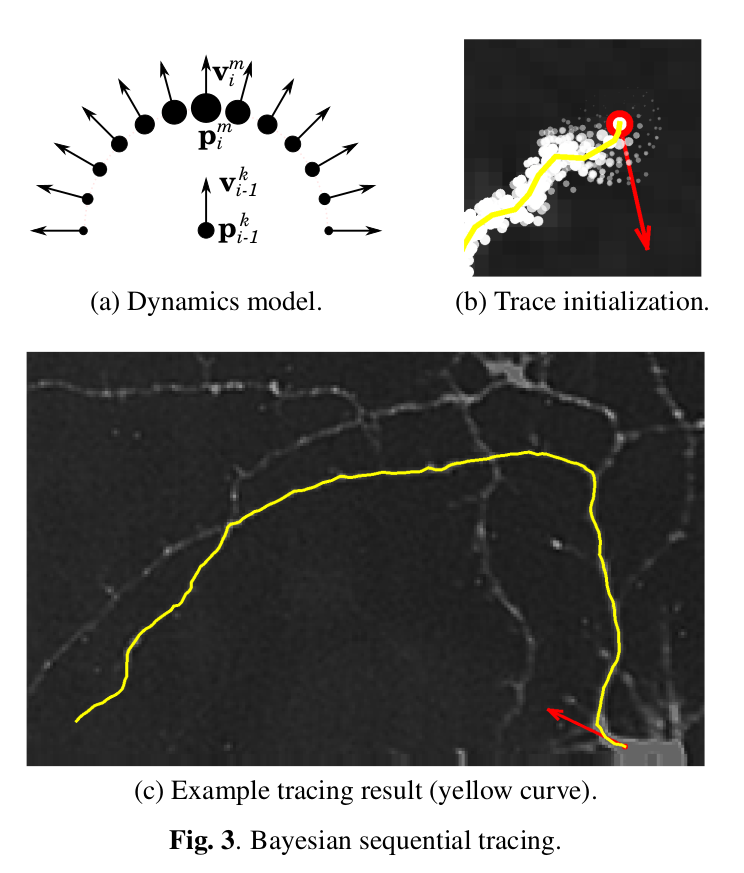
\includegraphics[height=3cm]{Images/bayesian_tracing.png}
  \label{fig:modele bayesien}
  \caption{Tracking, fluoroscopy}
\end{figure}

% Modèles géométriques
Les modèles d'intensités ne prennent pas en compte la forme des objets détectés et peuvent ainsi détecter des objets de même intensités d'étant pas des vaisseaux. Par exemple, pour des vaisseaux faiblement contrastés et bruitées, la distribution d'intensité des vaisseaux risque de chevaucher la distribution du bruit.

\begin{figure}
  \centering
  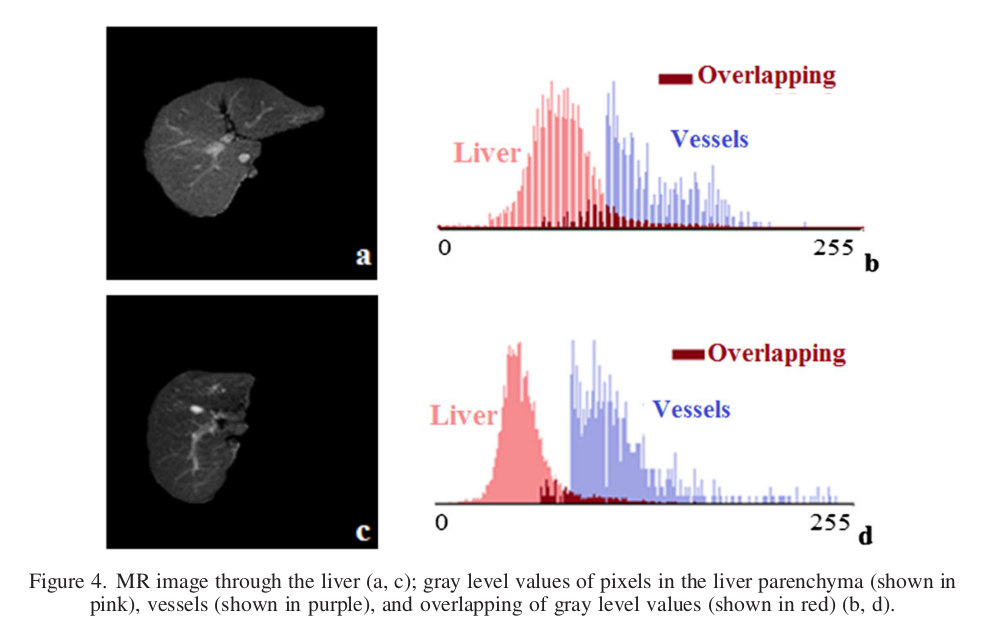
\includegraphics[height=5cm]{Images/Goceri[2016].png}
  \label{fig:overlap_vessels_tissues}
  \caption{Histogrammes d'intensité des tissues du foie, en bleu l'intensité des vaisseaux, en rouge l'intensité des tissues du foie (image placeholder, Goceri[2016] ) }
\end{figure}

Les modèles géométriques viennent compléter les modèles d'intensités. En effet, l'aspect spécifique des vaisseaux qui forment des structures curvilignes, les rendent le plus souvent très différents des autres organes.

Les modèles les plus basiques sont les modèles en forme de disques, ou sphériques pour leurs équivalents 3D \cite{Law2008_OOF}. Les modèles sphériques sont limités par le fait que les éléments sphériques et tubulaires ne sont pas dissociables. Des variantes cylindriques ont aussi été proposées dans la littérature, Esneault \cite{Esneault2009_moments_graph_cut}, Cetin \cite{Cetin2015_high_order}. Le modèle prédominant est le modèle tubulaire  développé dans le chapitre CH.\ref{} Celui-ci a l'avantage d'être plus général et flexible que le modèle cylindrique.

La litterature propose aussi un ensemble de modèles déformables, sans à priori de formes. Ceux-ci nécessitent le plus souvent un point d'initialisation donné manuellement ou déterminé de manière automatique. Ces modèles sont contraints par une énergie qui définie les limites de déformation du modèle. La difficulté principale est de trouver un terme de contrainte permettant d'éviter un écoulement du modèle hors des vaisseaux.

Enfin, une famille de modèle provenant de la morphologie mathématique modélise les vaisseaux comme un ensemble de chemins curviliénaires.\cite{Heijmans2005_path_opening}

\begin{figure}
  \centering
  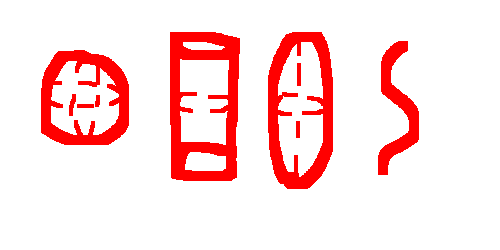
\includegraphics[height=5cm]{Images/geometricModels.png}
ap  \label{fig:geometricModels}
  \caption{Modèles géométriques basiques, sphère, cylindre, tubulaire et curvilinéaire}
\end{figure}

Enfin, les modèles à base d'atlas sont des modèles construis à base de mesures préalables. Ils sont construit en amont de la méthode de segmentation et représentent une connaissance ``en moyenne'' d'un modèle géométrique, d'intensité ou plus fréquement d'une localisation dans l'espace. Les modèles d'atlas sont particulièrement adaptés à des structures rigides qui présentent peu de diversités anatomiques.

\subsection{Segmentation deep learning 3D}
\label{sec:EA:segmentation_deep3D}

A partir de 2015, les réseaux de neurones ont pris une place prépondérante dans la litterature de la segmentation, grâce à l'apparitions des modèles de réseaux profonds, de l'augmentation de la puissance de calculs et d'un nombre important de données annotées. Pour le médicale cette installation se fait de manière plus lente mais assurée. La classification  modèle, caractéristiques, schéma d'extraction est plus complexe à appliquer en deep learning. Celui-ci repose sur trois éléments, l'architecture du réseau, les données d'entrées et les vérités terrains associées, le critère de convergeance du réseau.

% Que le médical
\subsubsection{Architecture}
% Architecture
% 1) Réseaux de neurones à convolution
% 2) Types d'entrainement, supervisé vs non supervisé
Les réseaux de neurones convolutifs ont pris une place prépondérante dans la littérature, en particulier pour le médical. Ces méthodes reposent sur l'apprentissage automatique de caractéristiques de l'image. Pour cela, un grand nombre d'exemples est montré au réseau, celui-ci va alors produire un résultat qui va être corrigé. Deux types d'entrainement sont principalement utilisés, l'entrainement supervisé avec des paires \{image d'entrée,vérité terrains\} et l'entrainement non supervisé avec des images d'entrées et une énergie à minimiser, permettant de contraindre la sortie du réseau. L'erreur de classification du réseau est ensuite propagée à travers chaque couches qui le compose par rétro-propagation du gradient d'erreur.

Les réseaux convolutionels sont une représentation compactes des réseaux historiques, les perceptrons multicouches, et ont en plus la propriété d'être invariant à la translation.
% 4) Publications milestones (AlexNet,VGG,ResNet,DenseNet,U-Net)
% 5) Variantes de Unet (Res-Unet,Vesselnet, branches multiples)
L'avenement des réseaux de convolution (CNN) commence avec AlexNet et VGG qui répondent à des tâches de classification sur des images naturelles (classification). Avec la création de réseaux de plus en plus profonds, l'entrainement se révèle de plus en plus difficile, notament à cause de la disparition du gradient au fur et a mesure des couches traversées. Ce problème a été résolu plus tard par le modèle ResNet, qui propose des ``skip connections'' afin d'introduire une redondance de l'information. De la même manière, le modèle DenseNet propose de réutiliser des caractéristiques tout au long du réseau, aliant redondance et légèreté du réseau.

C'est l'architecture d'auto-encodeur U-Net qui a percé dans le milieu médical en permettant de segmenter de manière précise des organes.
% 6)

\todo{Citer les papiers avec U-net}
\todo{Introduire les fonctions de coût}
\todo{Parler du besoin crutial de données}
\todo{Parler des limitations en lien avec le foie, notamment l'IRM, ou le faire dans la partie bilan}

\section{Rehaussement}
\label{sec:EA:rehaussement}
\subsection{Introduction}
\label{sec:EA:rehaussement:introduction}

Parmis les méthodes de segmentation des vaisseaux sanguins, une grande majorité utilise une étape de pré-traitement, consistant à faciliter la segmentation des vaisseaux en augmentant de manière significative leur contraste et en atténuant le signal de toutes les autres structures. Ces filtres portent le nom de ``filtres de rehaussement de vaisseaux'' (vesselness filters, traduit litéralement : ``filtres de vaiseaux-sité''). Ces filtres combinent des modèles d'intensités et de géométries spécifiques aux vaisseaux avec des descripteurs d'images. De par leur positionnement en amont des pipelines de segmentation, ils ont une influence directe sur le choix et les performances des schémas d'extractions.

\begin{figure}
  \centering
  
\includegraphics[height=4cm]{Images/img_required.jpg}
  \label{fig:placeholder}
  \caption{placeholder}
\end{figure}

Un filtre de rehaussement peut se baser sur plusieurs stratégies pour améliorer le signal des vaisseaux :

\begin{itemize}
\item la distribution des intensités
\item la géométrie des structures
\item la hiérarchie des structures
\end{itemize}

En effet, pour la tomodensitométrie comme pour l'IRM, certaines hypothèses physiques sont applicables aux vaisseaux.

Premièrement, pour l'angiographie avec injection d'agent de contraste, on considère que les vaisseaux ont une intensité supérieure aux tissues qui les entournent. Cette hypothèse, bien que souvent vraie, se retrouve limitée en pratique. En effet, cette hypothèse dépend des conditions liées au temps d'acquisition et de la vascularisation de l'organe étudié. Plus l'acquisition est longue et les échanges vasculaires nombreux dans l'organe, plus l'agent de contraste se diffuse dans celui-ci. Ce processus peux aller jusqu'à rendre l'organe totalement uniforme sans possibilité de différencier les tissues qui le compose. Comme discuté dans la section SEC. ~\ref{sec:contexte:images} du chapitre CH.~\ref{} l'utilisation d'agent de contrastes ne garanti pas un aspect uniforme des vaisseaux. Cet aspect varie en fonction de la concentration de l'agent de contraste dissous dans le sang. Par conséquent, plus le diamètre des vaisseaux est réduit, plus la concentration, et donc le contraste, est faible. Pour des tronçons de vaisseaux de même taille, la viscosité du sang ou la géométrie des vaisseaux peut aussi faire s'accumuler l'agent de constrate dans des régions spécifiques.

Une fois l'hypothèse d'intensité posée, on peut établir de nouvelles hypothèses sur la géométrie des vaisseaux. L'hypothèse la plus courante est d'asimiler les vaisseaux à des cylindres ou des tubes soumis à des contraintes géométriques plus ou moins relachées. Cette hypothèse peut se montrer suffisante lorsque l'on ne considère qu'un seul tronçon de vaisseaux. En réalité, dans un réseau vasculaire, chaque tronçons peut avoir des formes et diamètres variés, et les tranches successives d'un même tronçon ne sont pas forcément homogène. De plus, les vaisseaux sont interconnectés entre eux, formant aux jonctions des objets géométriques qui sortent du cadre des hypothèses initiales.

Enfin, on peut établir des hypothèses basées sur la hiérarchie des vaisseaux. La plupart du temps, les organes sont alimentés par un ou des vaisseaux rincipaux, les artères, relativement larges qui se subdivisent ensuite pour alimenter les différentes régions de l'organe. Cette subdivision prend la plupart du temps la forme d'une bifurcation, c'est à dire un vaisseaux se séparant en deux vaisseaux (pour les artères, et inversement pour les veines). Plus rarement, on peut observer des N-furcations, comme la trifurcation de la carotide. Cette division des vaisseaux est la plupart du temps accompagnée d'un changement de diamètre qui dépend du sens du flux sanguin. Dans certains organes, on peut ainsi vérifié des propriétés topologiques. Par exemple pour le foie, le réseau vasculaire porte peut être assimilé à un graph sans cycle, voir à un arbre dont les noeuds sont les bifurcations et les arêtes les vaisseaux.

\begin{figure}
  \centering
  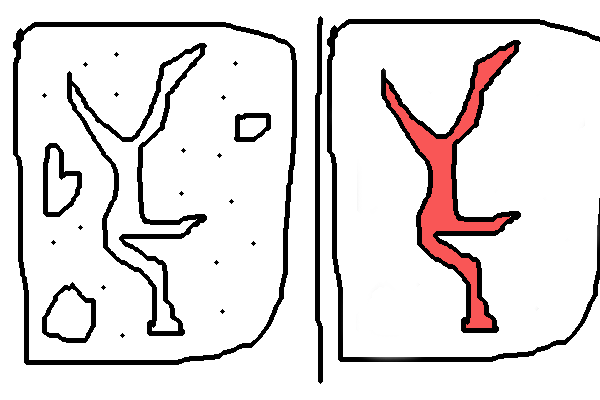
\includegraphics[height=5cm]{Images/example_enhancement.png}
  \label{fig:exemple_vesselness}
  \caption{exemple de filtre de rehaussement de vaisseaux}
\end{figure}

\section{Espace d'échelle}
\label{sec:EA:rehaussement:echelle}


La détection d'un réseau vasculaire dans sa totalité implique de détecter des vaisseaux de différentes tailles. En effet, les plus gros vaisseaux peuvent faire plusieurs dizaines de voxels de diamètres tandis que les vaisseaux les plus fins, atteignants les limites de la résolution des capteurs, peuvent  mesurer jusqu'à un voxel de diamètre. Il n'est pas envisageable de ré-écrire un algorithme pour chaque taille de vaisseaux, c'est pourquoi des cadres théoriques, appelés \emph{espace d'échelle} ont été formulés. Ces espaces d'échelles permettent d'établir un cadre uniforme pour sélectionner les structures d'une image à une échelle donnée. Trois espaces d'échelles sont courament associés au réhaussement de vasculaire dans la litterature : L'espace d'échelle gaussien, l'espace d'échelle granulométrique et l'espace d'échelle de flux orienté.

\subsection{Espace Gaussien}
\label{sec:EA:rehaussement:echelle:gaussien}

% what we want to say
% why gaussian ?
% - smoothing remove lower structures without introducing new ones
% - relation between sigma and sizes
% - relation to sigma and vessels radius
Lindenberg introduit la théorie de l'espace d'échelles gaussien dans \cite{lindeberg2013_scale}. Dans cette théorie, a l'échelle la plus basse, la totalité des structures sont présentes, et les détails les plus fins sont présents. Au fur et à mesure que l'échelle augmente, les détails sont lissés pour ne laisser que les maximas locaux correspondants aux formes les plus grandes. Ainsi, l'échelle minimale correspond à l'image initiale et l'échelle maximale correspond à une image uniforme. Il a été démontré que les noyaux gaussien étaient les seuls noyaux permettant de passer d'une échelle fine à une échelle grossière sans provoquer l'apparition de nouvelles structures. De plus, un mécanisme identique a été observé dans le fonctionnement du champ visuel.

\begin{figure}
  \centering
  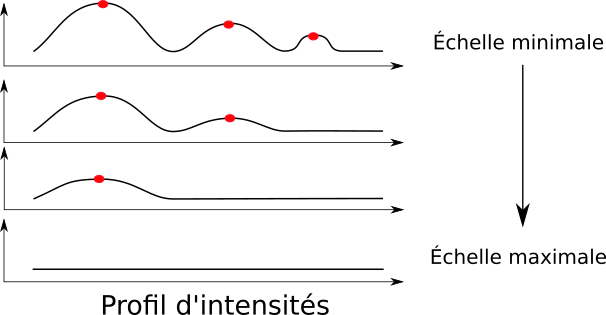
\includegraphics[height=5cm]{Images/gaussian_smoothing.png}
  \label{fig:gaussian_smoothing}
  \caption{Lissage gaussien, les structures de taille égales ou supérieures à $\sigma$ sont conservées alors que les structures de taille inférieures disparaissent}
\end{figure}

\begin{equation}
  gauss(x,y,\sigma_{x},\sigma_{y}) = \frac{1}{ \sigma\sqrt{2\pi} }exp(-\frac{x^2 + y^2 + z^2}{2(\sigma_{x}+ \sigma_{y}+ \sigma_{z}) })
\end{equation}

La sélection de l'échelle dans un espace gaussien se fait par le choix de l'écart-type $\sigma$ de la gaussienne. La plupart du temps on considère un espace d'échelle uniforme, $\sigma_x = \sigma_y = \sigma_z$. Il faut noter que pour un $\sigma$ donné, la taille des structures n'est pas supérieure ou égale à $\sigma$ mais plutôt supérieure ou égale à $\alpha\sigma$. En effet, en empruntant le formalisme des statistiques, l'interval de confiance, c'est-à-dire la couverture d'une distribution normale, correspond à $34.1\%$ pour $\sigma=1$, $68\%$ pour $\sigma=2$ et $99.7\%$ pour $\sigma=3$. Ainsi, pour $\sigma=1$ on détectera des objets de rayon $3\sigma$ et de diamètre $6\sigma$.  

\begin{figure}
  \centering
  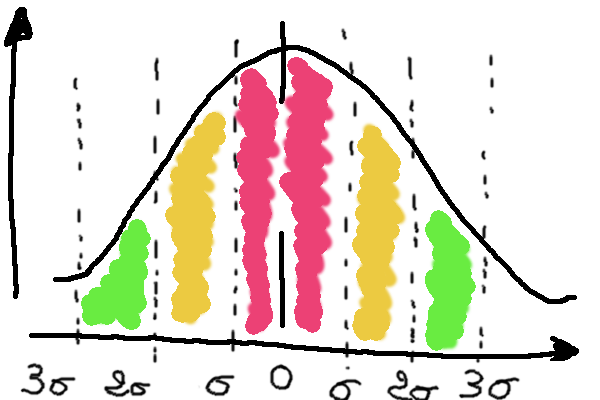
\includegraphics[height=5cm]{Images/normal_distribution_probability_coverage.png}
  \label{fig:normal_distribution_probability_coverage}
  \caption{couverture d'une distribution normale}
\end{figure}

L'espace gaussien se prète particulièrement bien à la modélisation des vaisseaux. En effet, la formulation de la gaussienne correspond bien à l'effet combiné des hypothèses de vaisseaux cylindriques et de la diminution d'intensité des vaisseaux au fur et à mesure que l'on s'éloigne de leur centre. En particulier pour un vaisseau parfait de diamètre $3\sigma$, les maximas locaux se situent le long de sa ligne centrale.

De plus, la gaussienne se prête très bien à une analyse locale de la géométrie basée sur la dérivation. Elle assure en effet les hypothèses de continuité du support de l'image et permet de combiner lissage et dérivation de l'image en une seule étape par dérivation du noyau gaussien.

Enfin, le lissage a l'avantage d'apporter une certaine robustesse au bruit et de compenser la perte locale de signal.

L'espace gaussien a toutefois des défauts. Le lissage de l'image implique nécessairement un étalement de toutes les structures qui peuvent par conséquent cacher des structures voisines de plus petites tailles. Ce phénomène est particulièrement observé lorsque plusieurs échelles sont étudiées. De même, deux structures adjacentes de même tailles peuvent fusionner, et ainsi créer une seule réponse, là où deux ojets existaient initialement.

\begin{figure}
  \centering
  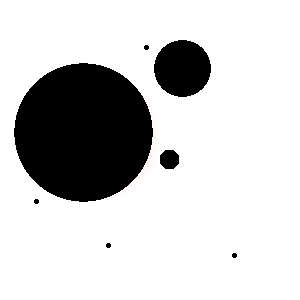
\includegraphics[height=3cm]{Images/gaussian_spilling_init.png}
  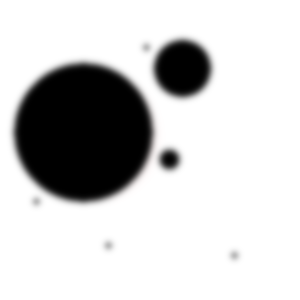
\includegraphics[height=3cm]{Images/gaussian_spilling_g10.png}
  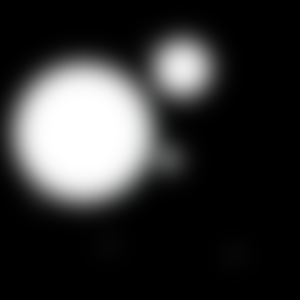
\includegraphics[height=3cm]{Images/gaussian_spilling_g40.png}
  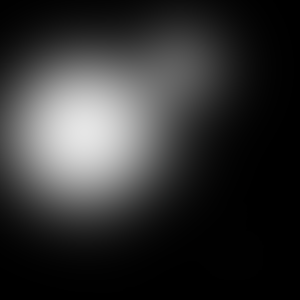
\includegraphics[height=3cm]{Images/gaussian_spilling_g100.png}
  \label{fig:scale_space_spilling}
  \caption{débordement du signal des structures larges sur les structures de plus petite tailles}
\end{figure}



\paragraph{Confirmation sur données réelles}

\todo{Expériences vérifiant en pratique la relation $3\sigma=diametre$}

\subsection{granulométrie}
\label{sec:EA:rehaussement:echelle:granulometrie}

La granulométrie est l'étude des tailles des particules d'un échantillon. En chimie, on utilise par exemple la technique du tamisage. Elle permet, grâce à un tamis et une grille dont on contrôle la taille du maillage, de ne conserver que des particules dont la taille est trop grosse pour passer à travers le tamis.

Un principe similaire est applicable en morphologie mathématique sur les images binaires et par extension en niveau de gris.

\subsubsection{Erosion et dilatation }

Deux opérations élémentaire, la dilatation et l'érosion, permettent de définir les opérations nécessaires pour définir un espace d'échelle morphologique. Les définitions qui vont suivre sont des opérations binaires relatives à des objets blancs sur fond noir.

\paragraph{Definitions}
% definition de Digital image processing, Gonzalez second edition, Mophology - p518
Soit deux ensembles définis dans $Z^3$ avec les composants $a=(a_1,a_2,a_3)$ et $b=(b_1,b_2,b_3)$.

La \emph{translation} de $A$ par $x = (x_1,x_2)$, noté $(A)_x$ est définie par :
% étrange cette formulation c|c non défini, idem pour x|x dans les autres.
\begin{equation}
  (A)_x = \{c|c = a+x, pour a \in A\}. 
\end{equation}

On définit la \emph{reflection} de B, dénoté $\widehat{B}$ par :

\begin{equation}
  (\widehat{B}) = \{x|x = -b, pour b \in B\}. 
\end{equation}

Le complémentaire de l'ensemble $A$ est défini par :

\begin{equation}
  (A^c) = \{x|x \not\in A\}. 
\end{equation}

La différence de deux ensemble $A$ et $B$, noté $A - B$, est défini par:

\begin{equation}
  (A-B) = \{x|x \in A, x\not\in \} = A \cap B^c.  
\end{equation}


\paragraph{dilatation}
En utilisant les propriétés précédentes, la dilatation s'exprime de la manière suivante :

\begin{equation}
 A \oplus B = {x|(\widehat{B}_x, \cap A \neq = \emptyset }
\end{equation}

La dilatation de $A$ par $B$ est l'ensemble de tous les déplacements de $\widehat{B}$ tel qu'il y ai au moins un pixel de recouvrement entre $A$ et $\widehat{B}$. Cette opération permet de faire grossir une structure en fonction de la forme de B.

\begin{figure}
  \centering
  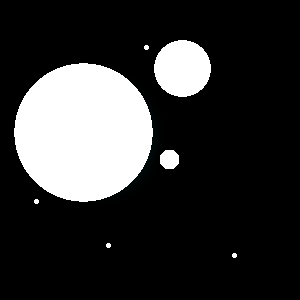
\includegraphics[height=3cm]{Images/morpho_init.png}
  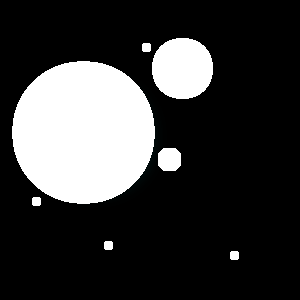
\includegraphics[height=3cm]{Images/morpho_dilate_k5.png}
  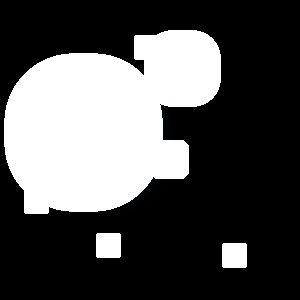
\includegraphics[height=3cm]{Images/morpho_dilate_k21.png}
  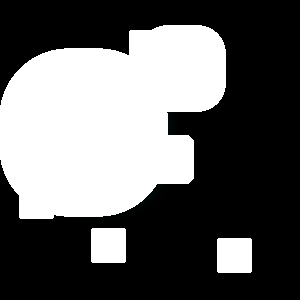
\includegraphics[height=3cm]{Images/morpho_dilate_k31.png}
  \label{fig:morpho_dilation}
  \caption{Exemple de dilatation}
\end{figure}

L'ensemble $B$ est courament appelé \emph{élement structurant}.

\paragraph{erosion}

L'opération oposée à la dilatation est l'érosion.

\begin{equation}
  A \ominus B = {x|(B)_x, \subseteq A}
\end{equation}

L'érosion de $A$ par $B$ est l'ensemble de tous les points $x$ tel que $B$ translaté de x est inclus dans $A$. 

\begin{figure}
  \centering
  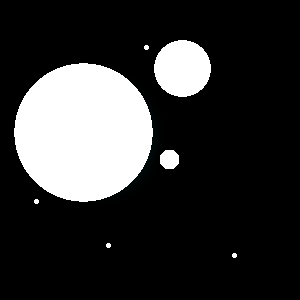
\includegraphics[height=3cm]{Images/morpho_init.png}
  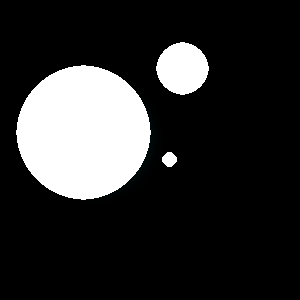
\includegraphics[height=3cm]{Images/morpho_erode_k5.png}
  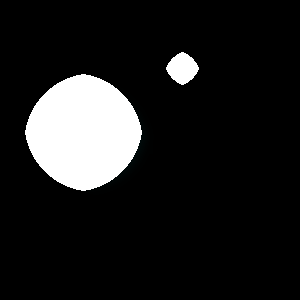
\includegraphics[height=3cm]{Images/morpho_erode_k21.png}
  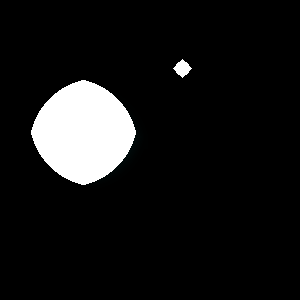
\includegraphics[height=3cm]{Images/morpho_erode_k31.png}
  \label{fig:morpho_erosion}
  \caption{Exemple d'érosion}
\end{figure}

\subsubsection{Fermeture et ouverture}

A partir des opérations d'érosion et de dilatation, on peut définir des opération composites, l'ouverture et la fermeture.

\paragraph{Fermeture}
L'ouverture est définie comme la dilatation de $A$ par $B$ suivi de l'érosion de $A$ par $B$.
\begin{equation}
 A \bullet B = (A \oplus B) \ominus B
\end{equation}

Cet opérateur est utilisé pour boucher les trous dont la surface est inférieure à la surface de l'élément structurant. L'érosion qui suit la dilatation permet d'assurer que la taille reste stable.

\begin{figure}
  \centering
  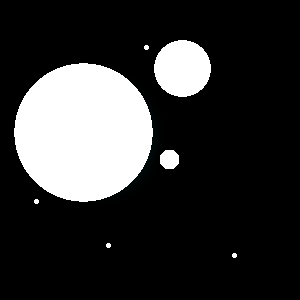
\includegraphics[height=3cm]{Images/morpho_init.png}
  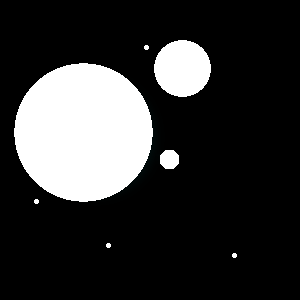
\includegraphics[height=3cm]{Images/morpho_close_k5.png}
  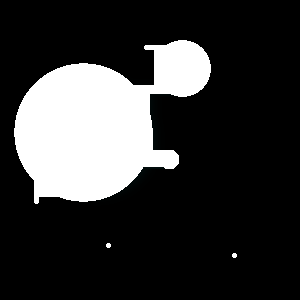
\includegraphics[height=3cm]{Images/morpho_close_k21.png}
  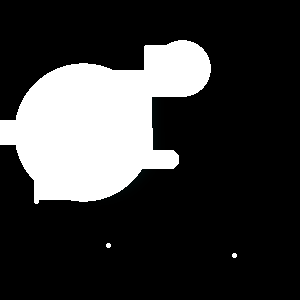
\includegraphics[height=3cm]{Images/morpho_close_k31.png}
  \label{fig:morpho_femerture}
  \caption{Exemple de fermeture}
\end{figure}

\paragraph{Ouverture}
L'ouverture est définie comme l'érosion de $A$ par $B$ suivi de la dilatation de $A$ par $B$.
\begin{equation}
 A \circ B = (A \ominus B) \oplus B
\end{equation}

\begin{figure}
  \centering
  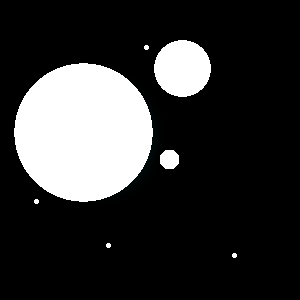
\includegraphics[height=3cm]{Images/morpho_init.png}
  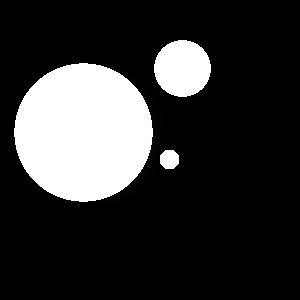
\includegraphics[height=3cm]{Images/morpho_open_k5.png}
  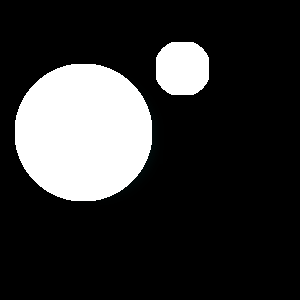
\includegraphics[height=3cm]{Images/morpho_open_k21.png}
  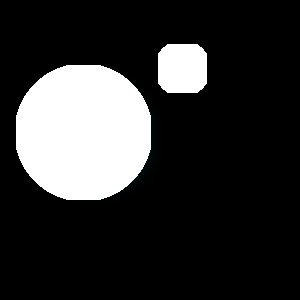
\includegraphics[height=3cm]{Images/morpho_open_k31.png}
  \label{fig:morpho_ouverture}
  \caption{Exemple d'ouverture}
\end{figure}

Cet opérateur est utilisé pour supprimer les structures de tailles inférieures à la surface de l'élément structurant. La dilatation qui suit l'érosion permet d'assurer que la taille des éléments restent stable.

L'ouverture permet de construire un espace d'échelle paramétré par la taille de l'élément structurant. Cet espace ne souffre pas d'une fusion parasite des structures adjacentes.

\subsection{Flux}
\label{sec:EA:rehaussement:echelle:flux}

Comme nous, l'avons vu dans la section SEC. \ref{sec:EA:rehaussement:echelle:gaussien}, l'espace d'échelle gaussien peut provoquer des débordements de structures sur d'autres, plus petites. On peut limiter se problème en utilisant un cadre différent, celui de l'analyse des flux.

Si l'on considère un champ de vecteur $V$, par exemple un fluide, ou un champ de gradient pour une image, on défini le flux passant à travers la surface $S$ orienté par sa normale $\vec{n_s}$ comme l'intégrale de la somme du produit scalaire entre le vecteur de flux $\vec{v}$ et la normale à la surface $\vec{n}$.

\begin{equation}
flux_S = \int_{S}< \vec{v},\vec{n} > d\rho
\end{equation}

On peut appliquer le calcul de flux à la surface d'un objet fermé. En particulier, des structures en forme de disques ou de sphères ont été particulièrement utilisées pour l'analyse de vaisseaux sanguins. On peut en effet contrôler directement le diamètre d'une sphère pour détecter les objets de la taille voulue. Cette formulation de l'échelle diffère des méthodes précédentes, car les objets tubulaires ne sont détectés que pour une échelle donnée, là ou les deux autres techniques conservent les objets à l'échelle donnée et aux échelles supérieures. Elle a aussi l'avantage de limiter l'analyse du flux à la surface de la sphère et donc de produire une réponse qui ne déborde pas.

La précision du calcul de l'intégrale de flux dépend du nombre d'échantillonages effectués sur $S$. Plus celui-ci est grand, plus le calcul est coûteux. De plus, plus l'échelle sélectionnée est grande, et donc plus la surface de la sphère est grande, plus le nombre d'échantillonage requis est important.

Law propose une formulation élégante du calcul de flux dans le domaine de Fourier afin de réduire drastiquement le temps de calcul par rapport à l'implémentation naïve \cite{law2009_efficient_implementation}.

Pour y parvenir, law propose d'exprimer le calcul de flux sous la forme d'une convolution dans le domaine temporel. L'avantage de la convolution est double, on évite l'étape d'échantillonage sur la surface et la convolution s'exprime comme une multiplication dans le domaine de Fourier. On peut exprimer le calcul de flux en terme de volume et non plus en terme de surface grâce au théorème de la divergence qui établit une égalité entre le flux à la surface d'un objet et le flux à l'intérieur de son volume. Ainsi :

\begin{equation}
  flux_{\partial C} = \int_{\partial C}< \vec{v},\vec{n} > d\rho \equiv \int_{C }\Delta I d\nu
\end{equation}

Plus précisément :

\begin{equation}
  f_s(x,y,z) = \int_{R_s}\vec{v}(x+t,y+p, z+q) . \vec{n}_{(t,p,q)}dA
\end{equation}

avec $R_s$ une région sphérique de rayon $s$; $dA$ une surface infinitésimale sur la surface $\partial R_s$; $\vec{n}_{(t,p,q)}dA$ le vecteur normal à $dA$ à la position $(t,p,q)$; et $\vec{v}$ le gradient de l'image $I$. $\vec{v}$ est obtenu à partir de l'image $I$ lissée par un noyau Gaussien afin d'assurer la dérivabilité du signal de $I$. $\vec{v}=\nabla(g*I)$.

Qui est équivalent à :

\begin{align}
  f_s(x,y,z) & = \int_{R_s} \vec{div}( \vec{v}(x+t,y+p, z+q) ) dtdpdq \\
  & = \int_{\omega} d_s(t,p,q) [\vec{div}( \vec{v}(x+t,y+p, z+q) )] dtdpdq
\end{align}

où $\omega$ est le domaine entier de l'image et $d_s(t,p,q)$ correspond à la fonction porte sphérique définie par :

\begin{equation}
d_s(x,y,z) = [\sqrt{x^2 + y^2 + z^2} \leq s]
\end{equation}

Ainsi, $f_s(x,y,z)$ peut être exprimé sous forme de convolution :
\begin{align}
  f_s(x,y,z) & = \int_{\omega} d_s(t,p,q) [\vec{div}( \vec{v}(x+t,y+p, z+q) )] dtdpdq \\
             & = \int_{\omega} d_s(t,p,q) (\Delta(g*I(x+t,y+p, z+q)))] dtdpdq \\
             & = \int_{\omega} d_s(-t,-p,-q) (\Delta(g*I(x+t,y+p, z+q)))] dtdpdq \\
             & = d_s * \Delta g * I(x,y,z) \\
             & = I * h_s(x,y,z) \\
\end{align}

avec $*$ l'opérateur de convolution, $\Delta$ l'opérateur laplacien.

Et dans le domaine de Fourier:

\begin{align}
  FFT( I * h_s(x,y,z) ) &= FFT(I) . H_s(u,v,w) \\
                       &= FFT(I) . [ (j2 \pi)^2 ( (\frac{u}{N_x})^2 + (\frac{v}{N_y})^2 + (\frac{w}{N_z})^2 ) ] \\
                       & . [ exp( -( (\frac{u}{N_x})^2 + (\frac{v}{N_y})^2 + (\frac{w}{N_z})^2 ) 2(\pi\sigma)^2 ) ]
\end{align}

\begin{figure}
  \centering
  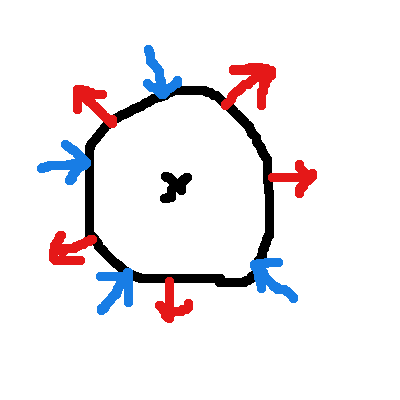
\includegraphics[height=6cm]{Images/flux.png}
  \label{fig:flux_sphere}
  \caption{flux sur la surface d'une sphère}
\end{figure}

\subsection{Multi-échelle}
\label{sec:EA:rehaussement:echelle:multiScale}

\todo{Voir si cette partie est à développer ici ou dans filtres, chapitre 4.}


\section{Familles de rehaussement}
\label{sec:EA:rehaussement:famille}

Plusieurs grandes familles de rehaussement sont présentes dans la littérature. 

\subsection{Morphologie}
\label{sec:EA:rehaussement:morpho}

Le rehaussement à base d'opérateurs morphologiques s'articule autour de deux familles, la composition d'éléments structurants rigides et l'utilisation de chemins curvilinéaires flexibles.

La composition d'éléments structurants rigides s'effectue la plupart du temps avec des boules et des cylindres. Les cylindres permettent de couvrir les parties curvilignes des vaisseaux, tandis que les boules couvrent les jonctions. Une composition d'ouvertures avec ces éléments est ensuite utilisée pour récupérer le réseau vasculaire. Sazak propose une schéma de ce type en 2 dimensions \cite{sazak_2D} puis en 3D \cite{sazak_3D} et compare son efficacité contre du rehaussement à base de tenseurs de phases et hessiens. Cette méthode bien que simple à mettre en pratique, nécessite plusieurs itérations avec des rotations des éléments structurants afin de capturer toutes les orientations des structures tubulaires. Cette méthode peut devenir coûteuse en 3D.

\begin{figure}
  \centering
  
\includegraphics[height=3cm]{Images/img_required.jpg}
  \label{fig:sazak_bowler_hat}
  \caption{bowler hat transform proposée par Sazak et al.}
\end{figure}

L'un des défaut de la méthode précédente est la rigidité des éléments structurants qui ne permettent pas toujours de capturer les variations de formes des vaisseaux. Hejimans \cite{Heijmans2005_path_opening} propose une famille d'éléments structurants flexibles dont la forme est définie par une grille d'adjacences. Des améliorations succesives de cet algorithme ont été proposés : XX propose une implémentation efficace de l'agorithm en O(XX), Cokelaer propose une version robuste au bruit en autorisant des discontinuités dans l'élément structurant, Merveille et al. itère en proposant un classement de l'orientation des chemins afin de segmenter les vaisseaux dans des images 2D et 3D.

\subsection{Phase}
\label{sec:EA:rehaussement:Phase}

% différents tensors, gradients,  

\subsection{Wavelets}
\label{sec:EA:rehaussement:wavelets}

% A voir comment articuler wavelets, noyaux gaussiens, etc.

\subsection{Hessienne}
\label{sec:EA:rehaussement:hessienne}

% Parler de la hessienne <-> co-occurence matrix et de leur explication géométrique. 
% parler des méthodes dont on ne traite pas par ailleur, Erdt, Li, etc.

\subsection{Diffusion}
\label{sec:EA:rehaussement:diffusion}

% VED
% HDCS

\section{Bilan et orientation des travaux}
\label{sec:EA:bilan}



